\documentclass{article}
\usepackage[utf8]{inputenc}
\usepackage[margin =1in,includefoot]{geometry}
\usepackage{indentfirst}
\usepackage{graphicx}
\usepackage{float}
\usepackage{caption}
\usepackage{subcaption}
% \usepackage{hyperref}

\title{Assignment 3 - COL334}
\author{Aayush Goyal}
\date{October 2021}

\begin{document}

\maketitle

\tableofcontents

\section{Changing different Congestion Protocols}

\subsection{For each protocol, generate a plot having Congestion window size on the y-axis and
time on the x-axis( till t=30s).}
The following 4 plots have been obtained for the the different congestion protocols that have been mentioned in the assignment statement. The protocols are:
\begin{enumerate}
    \item Tcp NewReno
    \item Tcp HighSpeed
    \item Tcp Veno
    \item Tcp Vegas
\end{enumerate}
\begin{figure}[H]
    \centering
    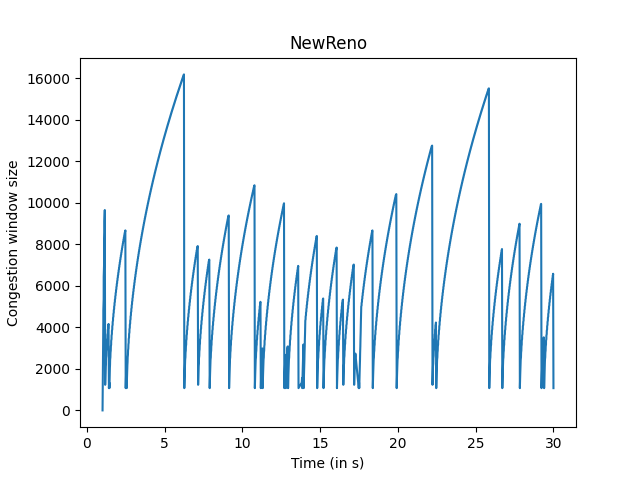
\includegraphics[scale = 0.8]{Q1/outputs/plots/NewReno.png}
    \caption{For the TCP New Reno protocol}
\end{figure}

\begin{figure}[H]
    \centering
    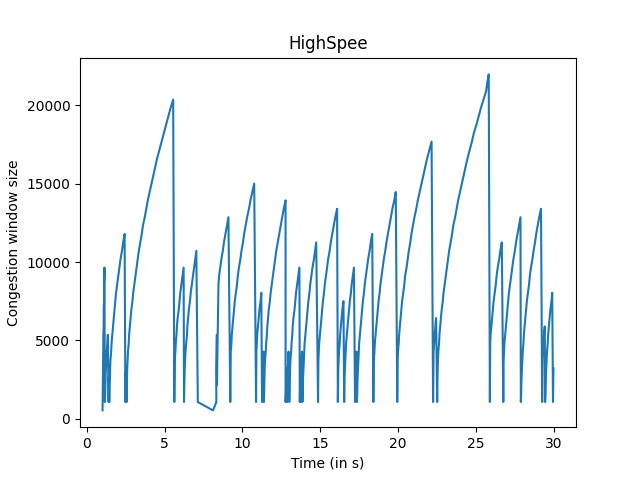
\includegraphics[scale = 0.8]{Q1/outputs/plots/HighSpee.png}
    \caption{For the TCP High Speed protocol}
\end{figure}

\begin{figure}[H]
    \centering
    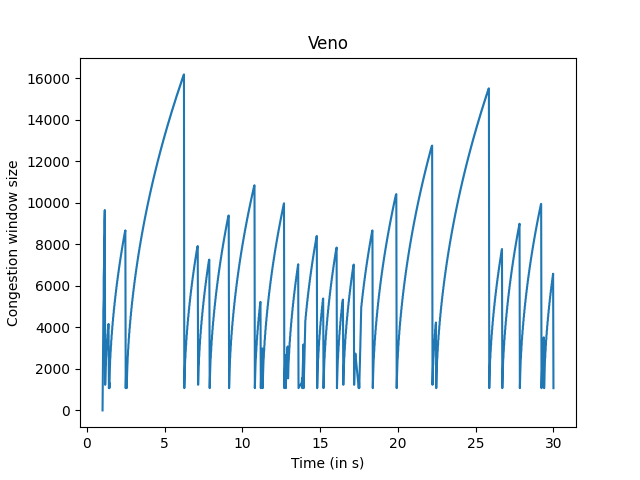
\includegraphics[scale = 0.8]{Q1/outputs/plots/Veno.png}
    \caption{For the TCP Veno protocol}
\end{figure}

\begin{figure}[H]
    \centering
    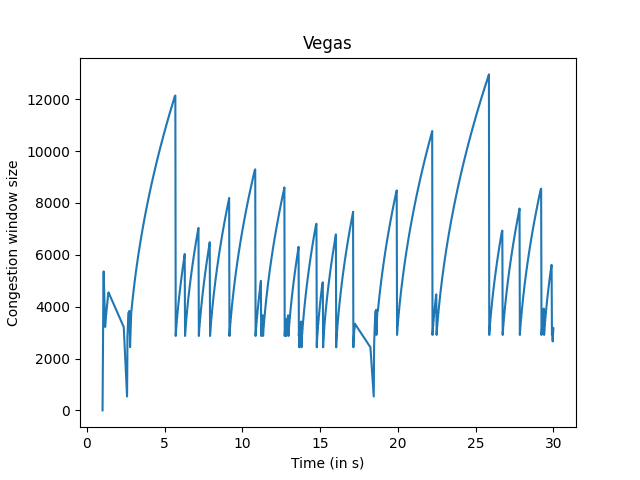
\includegraphics[scale = 0.8]{Q1/outputs/plots/Vegas.png}
    \caption{For the TCP Vegas protocol}
\end{figure}


\subsection{For each protocol, find the number of dropped packets in total. What is your
inference?}
\begin{enumerate}
    \item Tcp NewReno: 38 
    \item Tcp HighSpeed: 38
    \item Tcp Veno: 38
    \item Tcp Vegas: 39
\end{enumerate}

% TODO: Writing the inferences is left


\subsection{For each protocol, describe what you observed (4-5 sentences per protocol is
enough). You can talk about the trend you observed in the above plot, the algorithms
they used for different phases etc.}

% TODO: Writing the inferences is left

\section{Changing different Data Rate and Application Data Rate}
\subsection{Changing the Data Rate}
The Application Data Rate is fixed to 2Mbps in this section.

\begin{figure}[H]
    \centering
    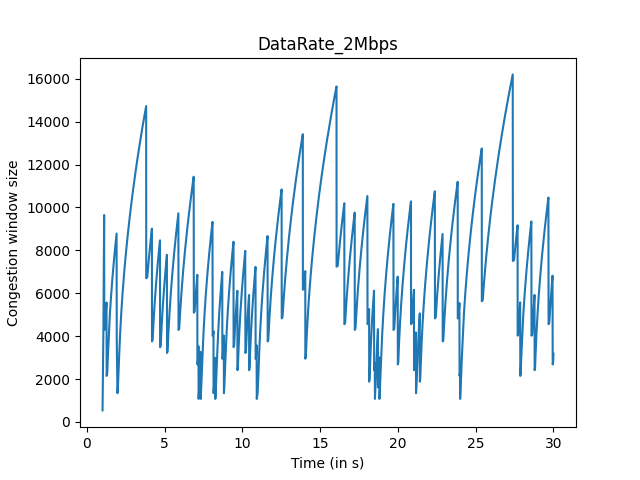
\includegraphics[scale = 0.8]{Q2/outputs/plots/DataRate_2Mbps.png}
    \caption{Data Rate has been fixed to 2Mbps}
\end{figure}

\begin{figure}[H]
    \centering
    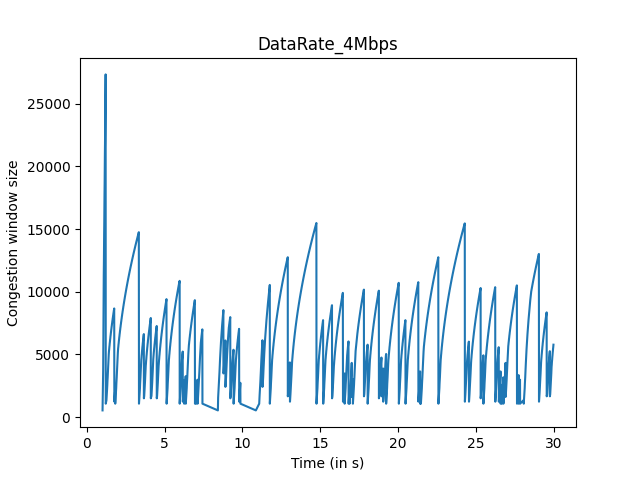
\includegraphics[scale = 0.8]{Q2/outputs/plots/DataRate_4Mbps.png}
    \caption{Data Rate has been fixed to 4Mbps}
\end{figure}

\begin{figure}[H]
    \centering
    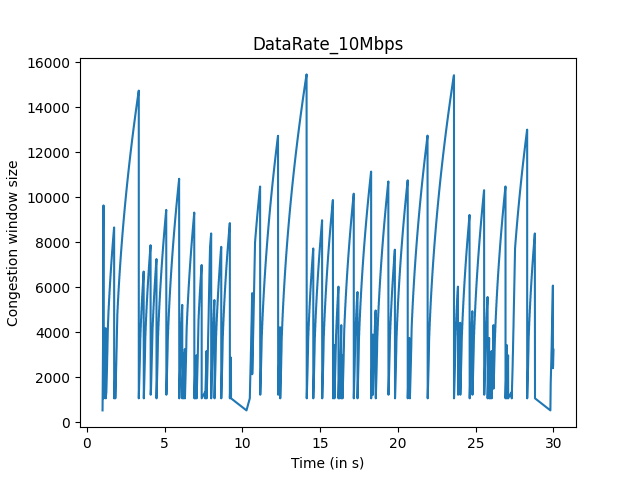
\includegraphics[scale = 0.8]{Q2/outputs/plots/DataRate_10Mbps.png}
    \caption{Data Rate has been fixed to 10Mbps}
\end{figure}

\begin{figure}[H]
    \centering
    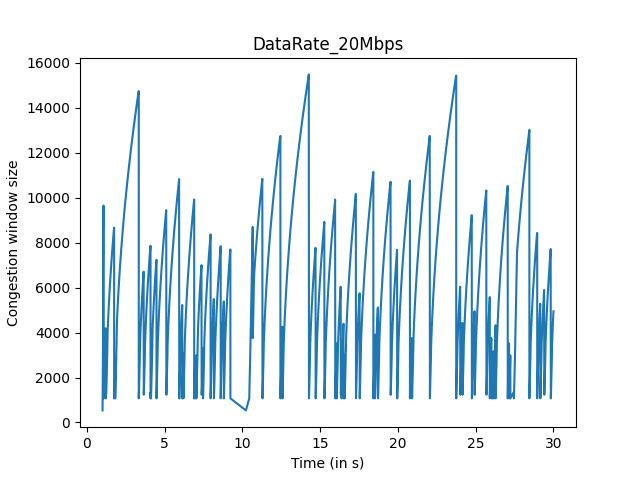
\includegraphics[scale = 0.8]{Q2/outputs/plots/DataRate_20Mbps.png}
    \caption{Data Rate has been fixed to 20Mbps}
\end{figure}

\begin{figure}[H]
    \centering
    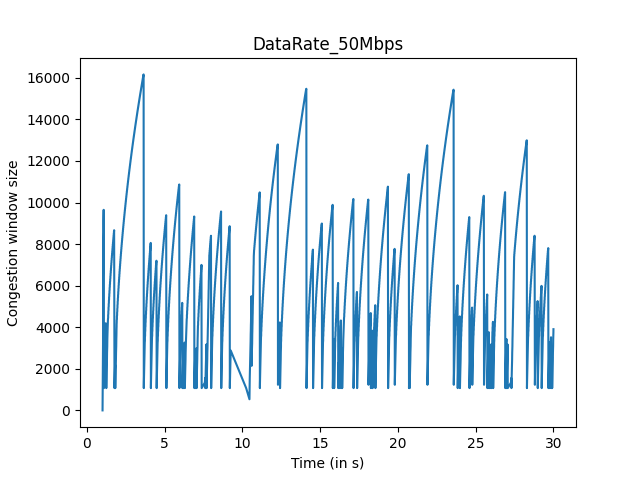
\includegraphics[scale = 0.8]{Q2/outputs/plots/DataRate_50Mbps.png}
    \caption{Data Rate has been fixed to 50Mbps}
\end{figure}


% TODO: Explaining the trends is left


\subsection{Changing the Application Data Rate}
The channel data rate has been fixed to 6Mbps in this part of the question.

\begin{figure}[H]
    \centering
    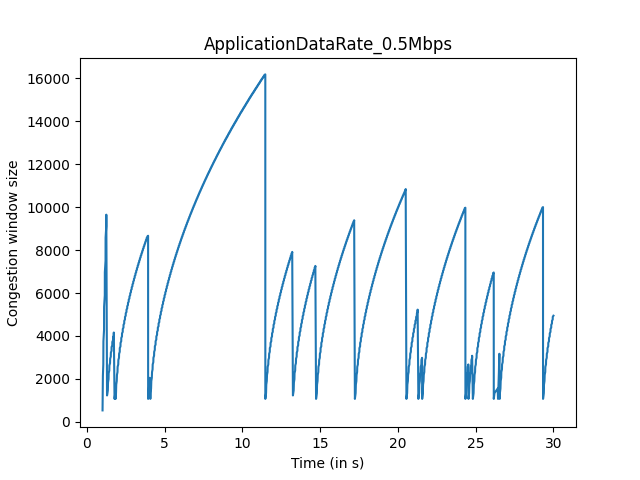
\includegraphics[scale = 0.8]{Q2/outputs/plots/ApplicationDataRate_0.5Mbps.png}
    \caption{Application Data Rate has been fixed to 0.5Mbps}
\end{figure}

\begin{figure}[H]
    \centering
    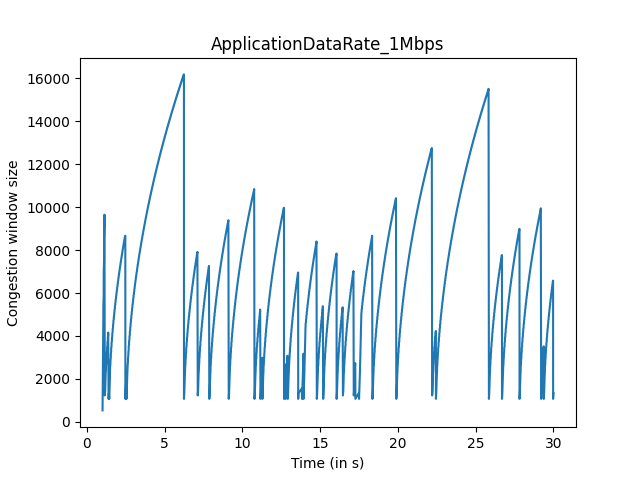
\includegraphics[scale = 0.8]{Q2/outputs/plots/ApplicationDataRate_1Mbps.png}
    \caption{Application Data Rate has been fixed to 1Mbps}
\end{figure}

\begin{figure}[H]
    \centering
    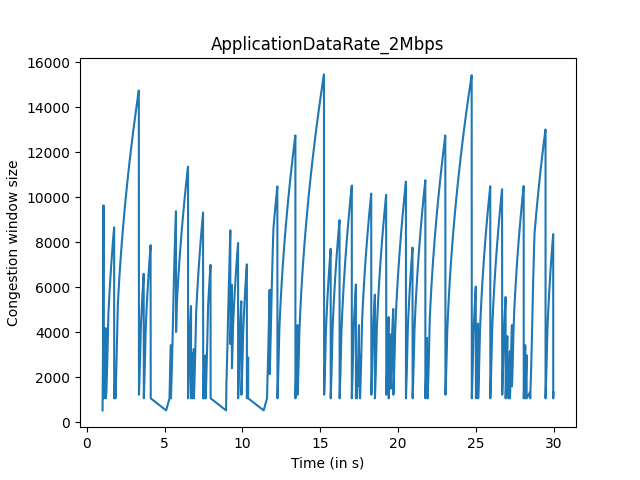
\includegraphics[scale = 0.8]{Q2/outputs/plots/ApplicationDataRate_2Mbps.png}
    \caption{Application Data Rate has been fixed to 2Mbps}
\end{figure}

\begin{figure}[H]
    \centering
    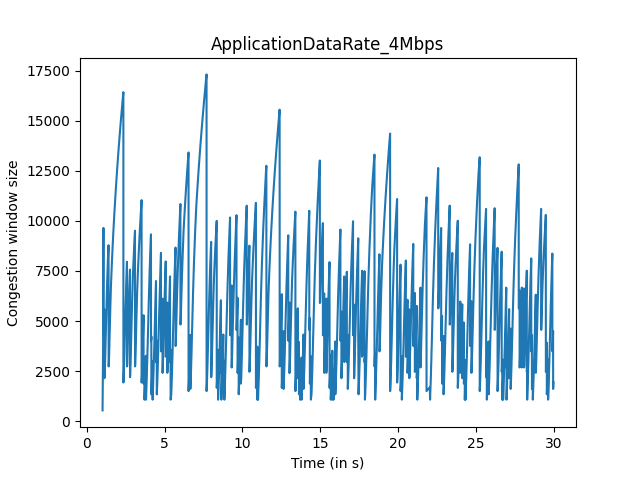
\includegraphics[scale = 0.8]{Q2/outputs/plots/ApplicationDataRate_4Mbps.png}
    \caption{Application Data Rate has been fixed to 4Mbps}
\end{figure}

\begin{figure}[H]
    \centering
    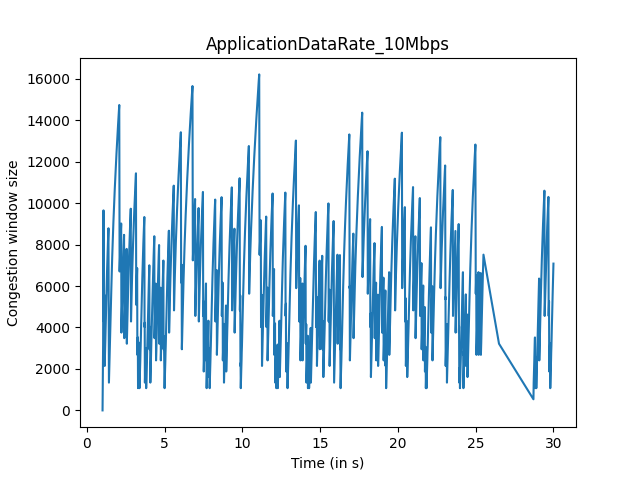
\includegraphics[scale = 0.8]{Q2/outputs/plots/ApplicationDataRate_10Mbps.png}
    \caption{Application Data Rate has been fixed to 10Mbps}
\end{figure}

% TODO: Explaining the trends is left

\section{Implementing TcpNewRenoCSE}

The files have been included with the submission which contain the code for SlowStart and Congestion Avoidance

\subsection{Plot Congestion window size vs time (from t=1 to t=30 seconds)}

\begin{figure}[H]
    \centering
    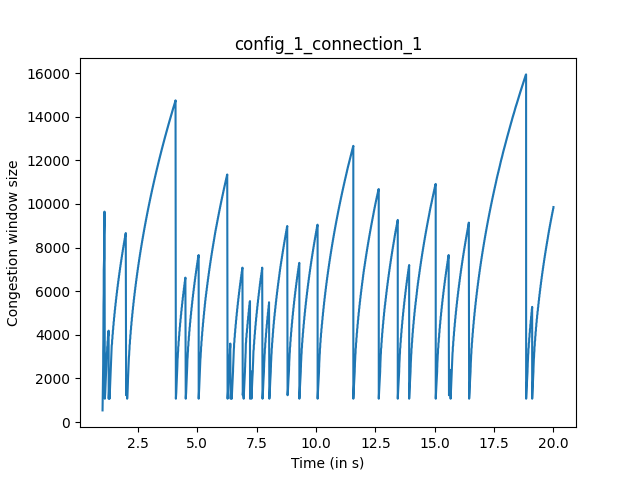
\includegraphics[scale = 0.8]{Q3/outputs/plots/config_1_connection_1.png}
    \caption{Plot for Configuration 1 and Connection 1}
\end{figure}

\begin{figure}[H]
    \centering
    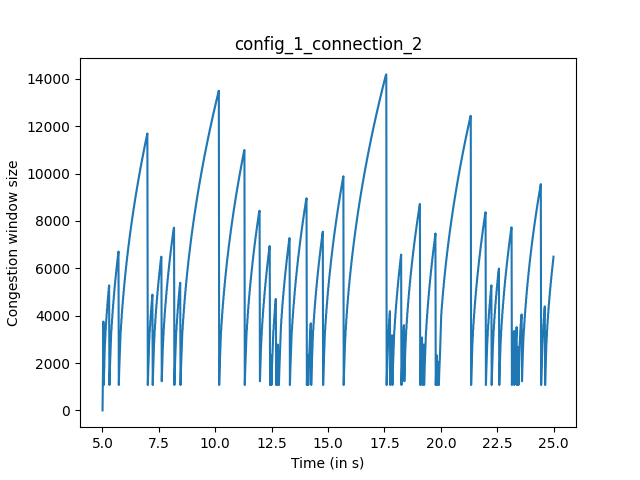
\includegraphics[scale = 0.8]{Q3/outputs/plots/config_1_connection_2.png}
    \caption{Plot for Configuration 1 and Connection 2}
\end{figure}

\begin{figure}[H]
    \centering
    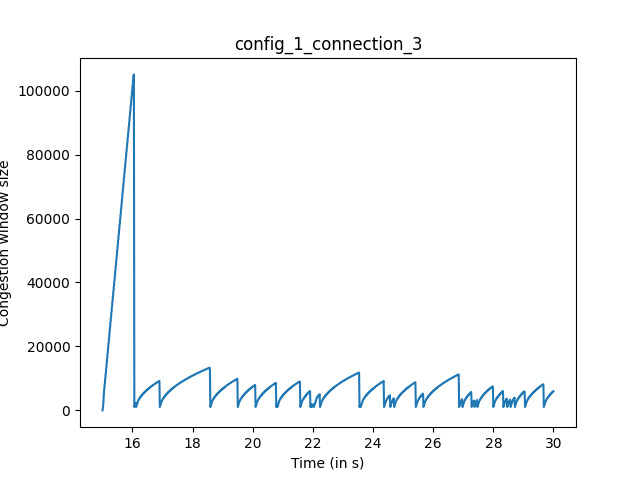
\includegraphics[scale = 0.8]{Q3/outputs/plots/config_1_connection_3.png}
    \caption{Plot for Configuration 1 and Connection 3}
\end{figure}

\begin{figure}[H]
    \centering
    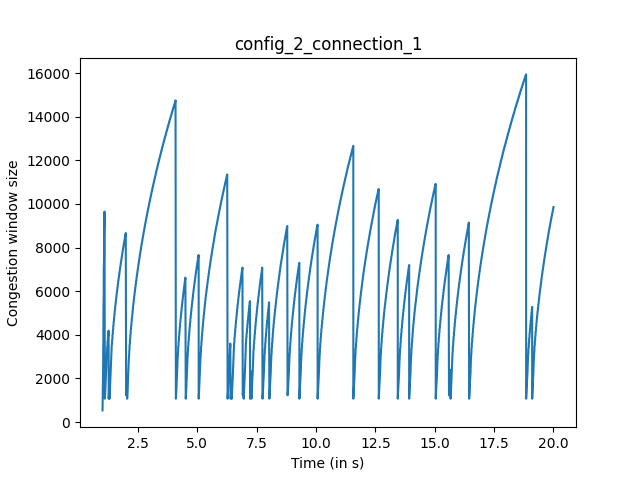
\includegraphics[scale = 0.8]{Q3/outputs/plots/config_2_connection_1.png}
    \caption{Plot for Configuration 2 and Connection 1}
\end{figure}

\begin{figure}[H]
    \centering
    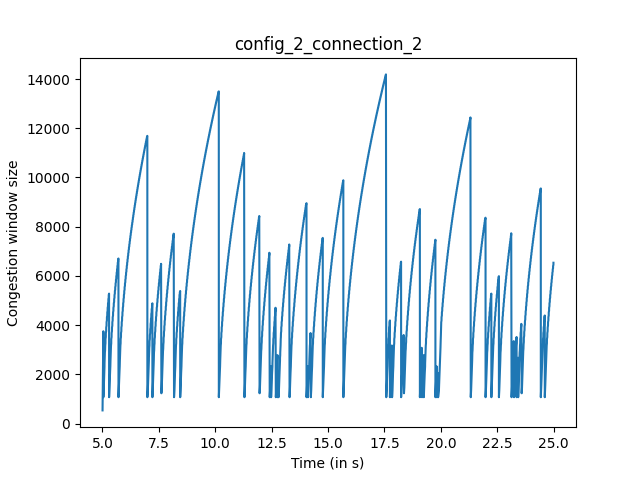
\includegraphics[scale = 0.8]{Q3/outputs/plots/config_2_connection_2.png}
    \caption{Plot for Configuration 2 and Connection 2}
\end{figure}

\begin{figure}[H]
    \centering
    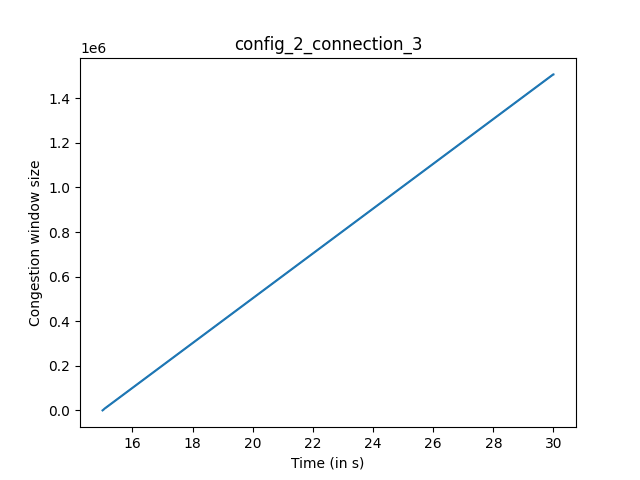
\includegraphics[scale = 0.8]{Q3/outputs/plots/config_2_connection_3.png}
    \caption{Plot for Configuration 2 and Connection 3}
\end{figure}

\begin{figure}[H]
    \centering
    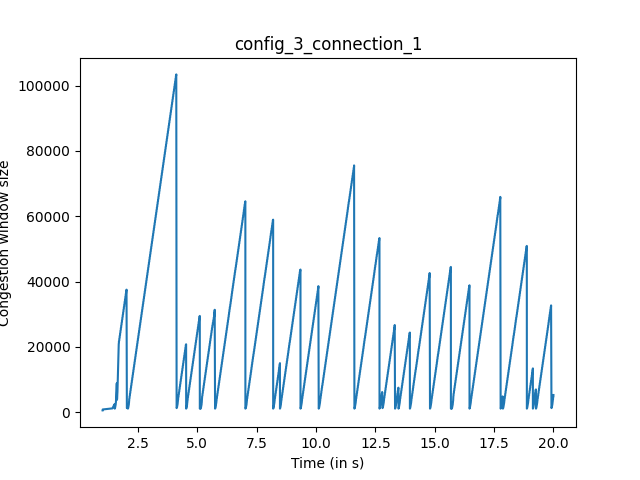
\includegraphics[scale = 0.8]{Q3/outputs/plots/config_3_connection_1.png}
    \caption{Plot for Configuration 3 and Connection 1}
\end{figure}


\begin{figure}[H]
    \centering
    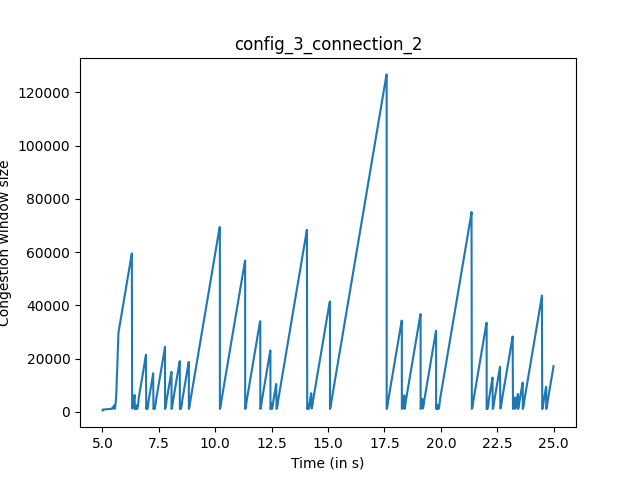
\includegraphics[scale = 0.8]{Q3/outputs/plots/config_3_connection_2.png}
    \caption{Plot for Configuration 3 and Connection 2}
\end{figure}

\begin{figure}[H]
    \centering
    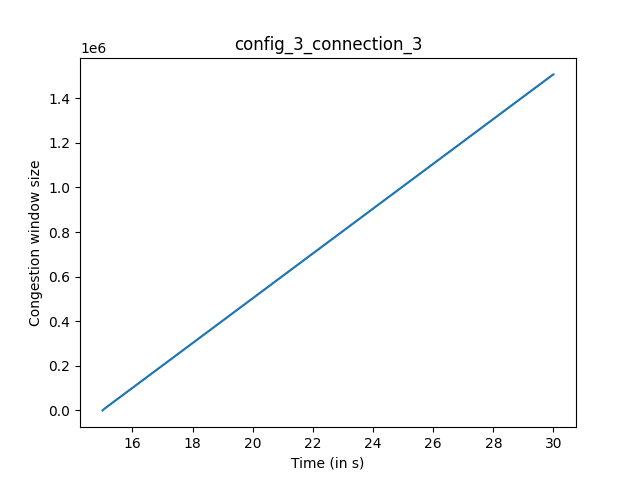
\includegraphics[scale = 0.8]{Q3/outputs/plots/config_3_connection_3.png}
    \caption{Plot for Configuration 3 and Connection 3}
\end{figure}

\subsection{Analyze the number of dropped packets for each connection separately.}

\begin{enumerate}
    \item Configuration 1: 113
    \item Configuration 2: 112
    \item Configuration 3: 110
\end{enumerate}

% TODO: Writing some ananlysis is left


\subsection{How does the congestion avoidance phase vary on the same sender when using
TCPNewRenoCSE vs TCPNewReno? Explain the observed trends. How does it
impact the entire network?}

% TODO: Writing what is asked in the above part


\section{Directory Structure}

As specified in the problem statement. I have submitted a plot.py, the instructions of how to use it have been given in the README.md. Apart from that the outputs have been stored in the following format, in the outputs folder of each question:
\begin{itemize}
    \item dropped: It contains the information regarding which how many packets have been dropped for a particular part
    \item toplot: This contains the time vs the old congestion window size vs the new window size. My plotting script takes all the files present in this and plots them.
    \item plots: This contains the plots. Look at the titles of the plots for information about them.
\end{itemize}
Further instructions on how to run have been given in the README.md in a well detailed manner.
\end{document}
